\section{Tijdsdilatatie vanuit wervel dynamiek}

We beschouwen een onzichtbare, rotatievrije superfluïde æther met stabiele topologische wervelknopen. Absolute tijd $t_{\text{abs}}$ stroomt met een constante snelheid, terwijl lokale klokken mogelijk een lagere snelheid ervaren als gevolg van drukgradiënten en knoopenergetica. Het Vortex Æther Model veronderstelt dat de snelheid waarmee tijd in het lokale frame (dichtbij de knoop) stroomt, afhangt van de interne hoekfrequentie $\Omega_k$. In deze sectie leiden we tijddilatatie-analogen af, geïnspireerd door de voorspellingen van de algemene relativiteitstheorie (GR), uitsluitend gebaseerd op druk- en vorticiteitsgradiënten in de vloeistof.

\begin{figure}[htbp]
\centering
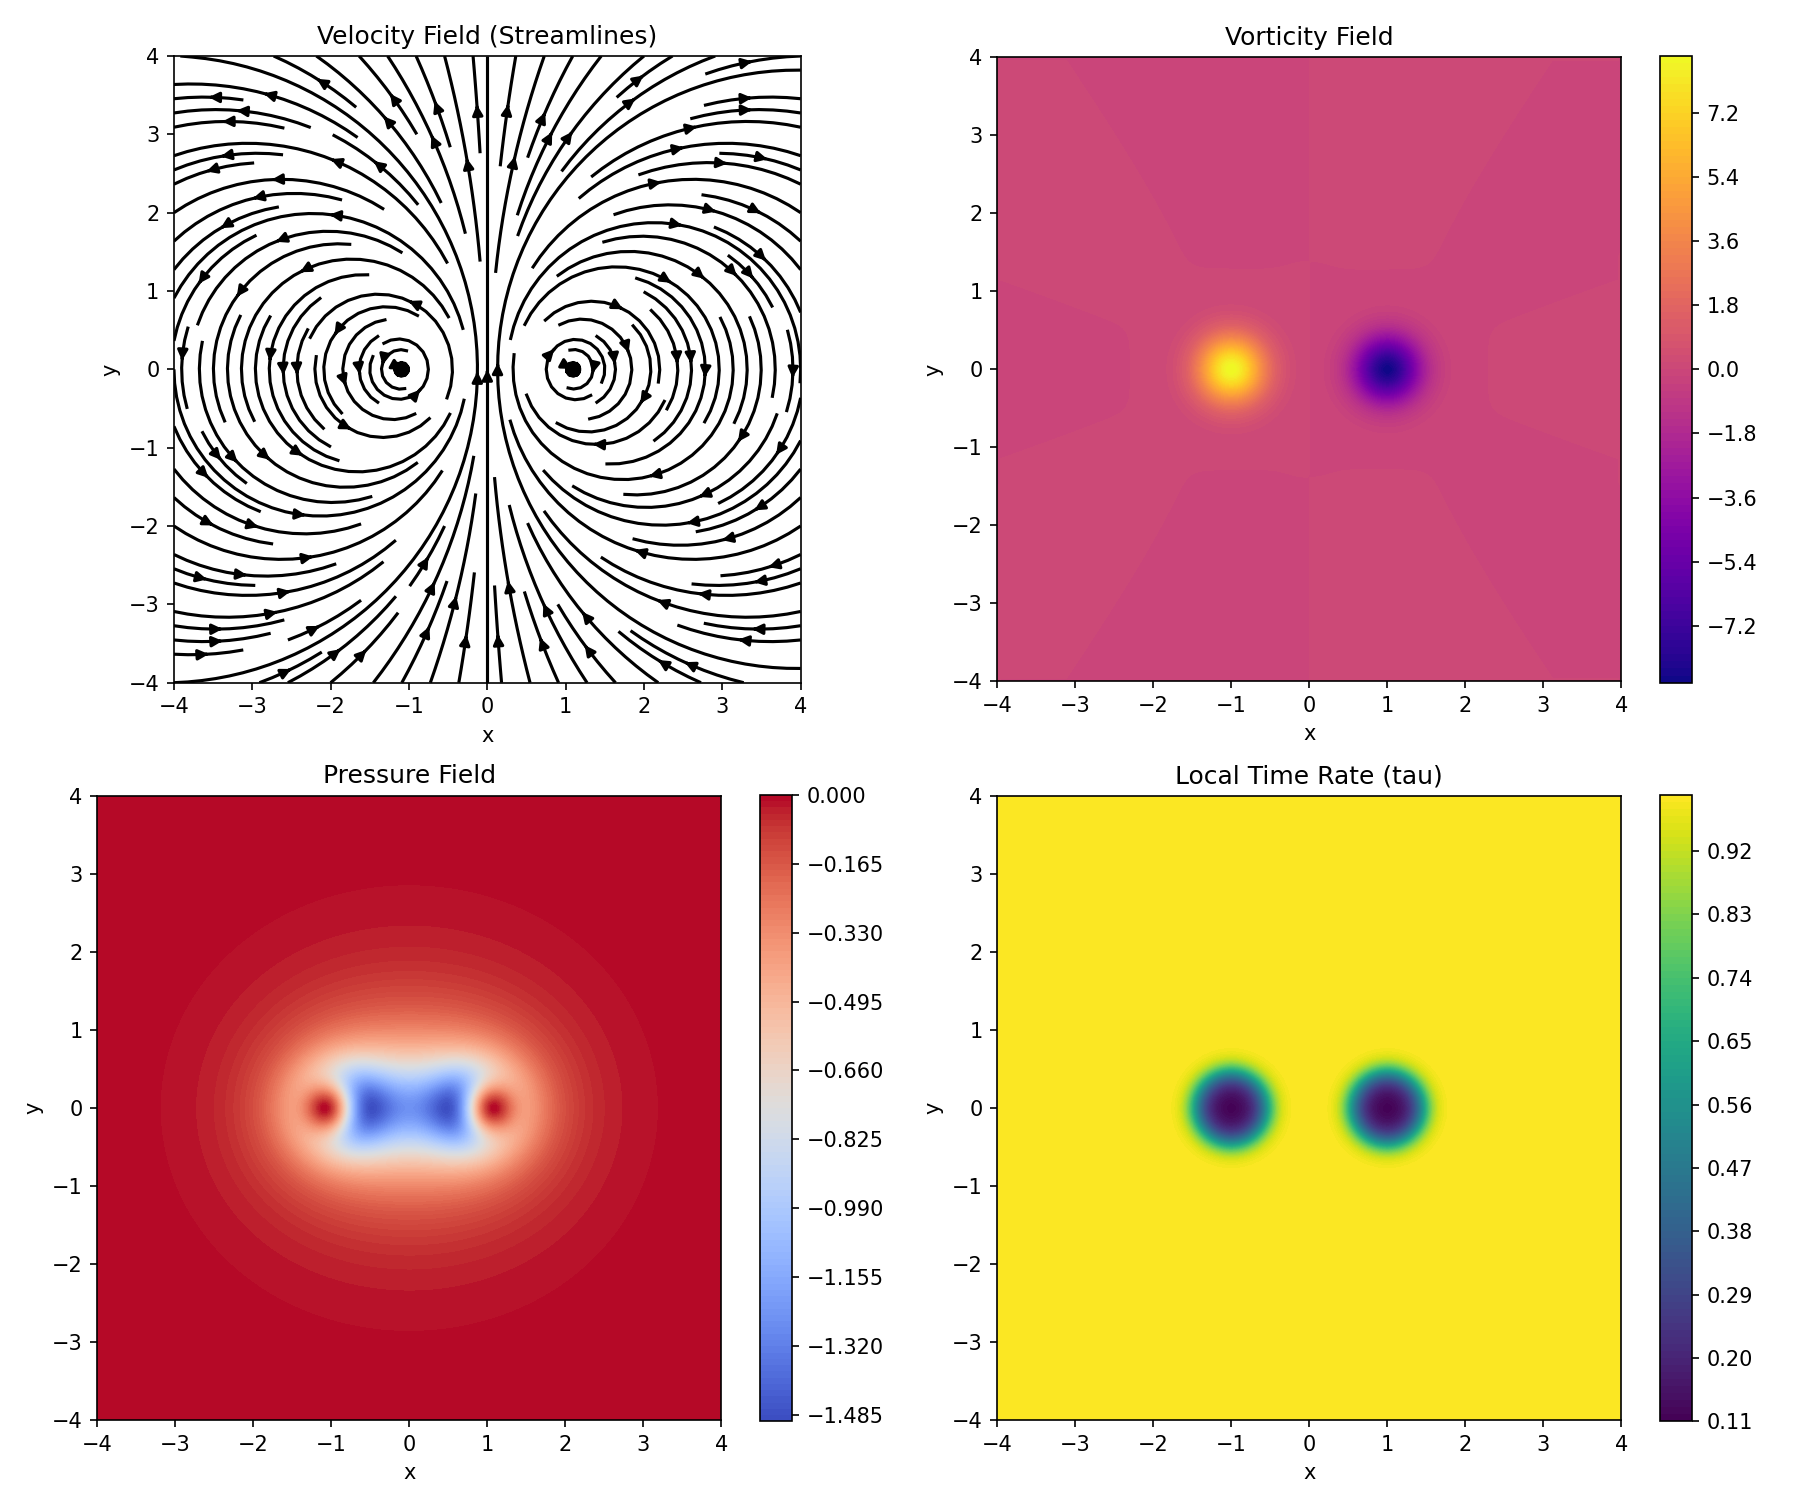
\includegraphics[width=0.85\textwidth]{streamlinesDiPole}
\caption{Snelheid stroomlijnt, vorticiteit, druk en lokale tijdsnelheid $\tau$ voor een gesimuleerd wervelpaar. Het drukminimum en de tijdvertraging komen duidelijk overeen met de gebieden met hoge vorticiteit. Dit illustreert direct de centrale bewering van het æthermodel: tijddilatatie volgt uit wervelenergetica en drukvermindering.}
\label{fig:vortexfields}
\end{figure}

In het Vortex Æther Model (VAM) ontstaat tijdsdilatatie niet vanuit de kromming van ruimtetijd, maar vanuit lokale wervel dynamica. Elk materiedeeltje is in VAM een wervel-knoopstructuur waarvan de interne rotatie (\textit{swirl}) de lokale klokfrequentie beïnvloedt.

De fundamentele koppeling tussen lokale wervel-snelheid en de lokale tijdsmeting volgt uit de Bernoulli-achtige relatie voor drukverlaging in stromingsvelden. De lokale klokfrequentie is gerelateerd aan de wervel-tangentiële snelheid $v_{\phi}(r)$ via de formule:
\begin{equation}\label{eq:vortex_tijdsdilatatie}
    \frac{d\tau}{dt} = \sqrt{1 - \frac{v_{\phi}^2(r)}{c^2}}
\end{equation}

Hierbij is $v_{\phi}(r)$ de tangentiële snelheid van het æthermedium op afstand $r$ tot het centrum van de wervel, en $c$ de lichtsnelheid. Dit is een directe analogie met de speciale relativistische snelheidsafhankelijke tijddilatatie, echter zonder ruimtetijdkromming en louter veroorzaakt door lokale rotatie van het æthermedium.

\subsection{Afleiding vanuit wervel hydrodynamica}

De afleiding volgt uit het Bernoulli-principe voor een ideale vloeistofstroming, gegeven door:
\begin{equation}\label{eq:Bernoulli}
    P + \frac{1}{2}\rho_{\ae} v^2 = \text{constant}
\end{equation}

Met wervel-stroming geïntroduceerd via vorticiteit $\vec{\omega} = \nabla \times \vec{v}$, definieert de lokale drukverlaging ten opzichte van de verre omgeving een lokale tijdvertraging. De lokale wervelsnelheid is gegeven door:
\begin{equation}\label{eq:tangentiele_snelheid}
    v_{\phi}(r) = \frac{\Gamma}{2\pi r} = \frac{\kappa}{r}
\end{equation}

waarbij $\Gamma$ de circulatieconstante is, en $\kappa$ het circulatiekwantum. Substitutie van \eqref{eq:tangentiele_snelheid} in \eqref{eq:vortex_tijdsdilatatie} geeft expliciet:
\begin{equation}\label{eq:vortex_tijd_expliciet}
    \frac{d\tau}{dt} = \sqrt{1 - \frac{\kappa^2}{c^2 r^2}}
\end{equation}

Hiermee is de tijdsdilatatie expliciet uitgedrukt in fundamentele wervel-parameters.

\subsection{Vergelijking met algemene relativiteit}

Ter vergelijking, in algemene relativiteit (GR) ontstaat gravitationele tijddilatatie uit ruimtetijdkromming, uitgedrukt door de Schwarzschildmetriek~\cite{schutz2009first}:
\begin{equation}\label{eq:GRtijd}
    \frac{d\tau}{dt} = \sqrt{1 - \frac{2GM}{rc^2}}
\end{equation}

De overeenkomsten en verschillen zijn direct zichtbaar: GR's gravitationele tijddilatatie is gerelateerd aan massa $M$ en gravitatieconstante $G$, terwijl VAM tijdsdilatatie puur hydrodynamisch is en direct verbonden met de lokale rotatiesnelheid van het æthermedium via wervel-circulatie $\kappa$.

\begin{figure}[ht!]
    \centering
    % Plaats hier een eigen grafiek of illustratie.
    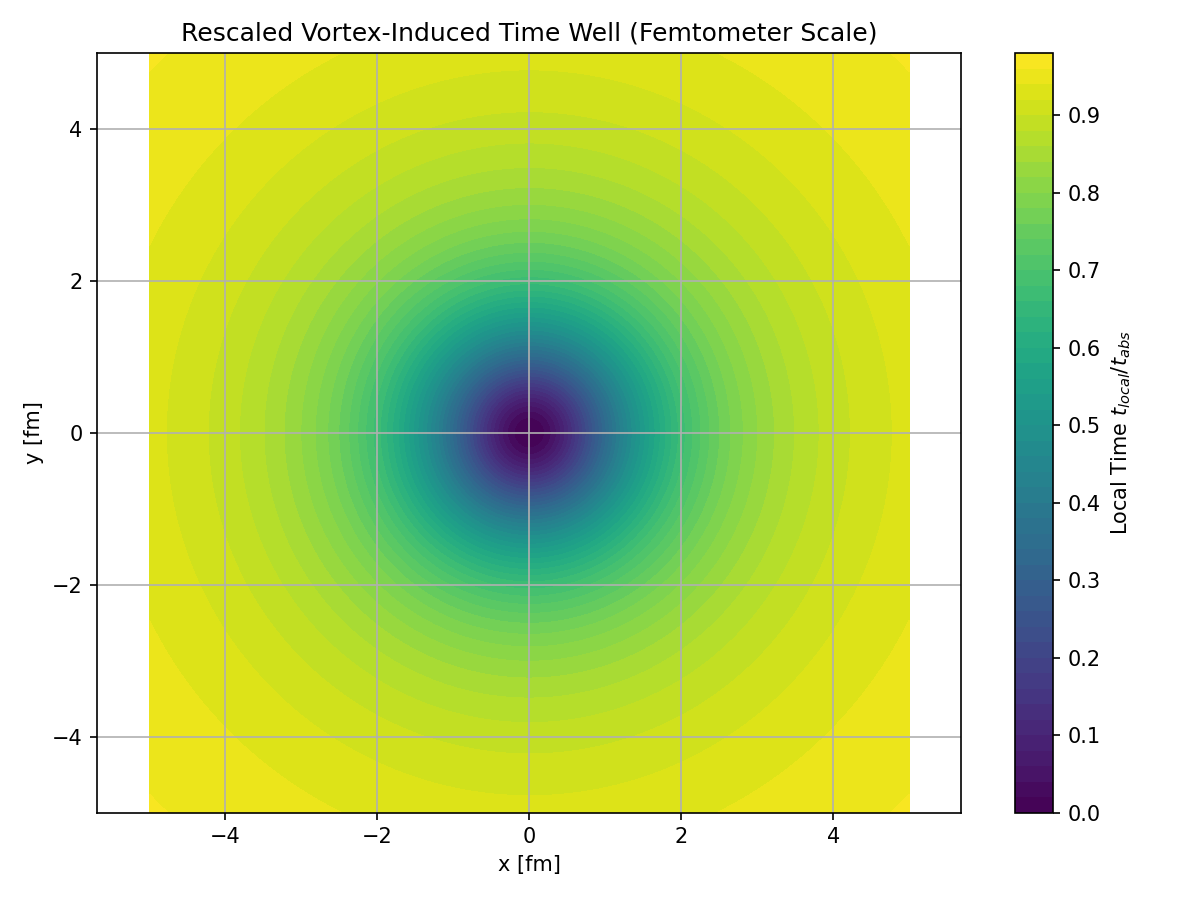
\includegraphics[width=0.7\linewidth]{RadialProfileOfLocalTimeDilation_Vortex-Induced_Time_Well}
    \caption{Vergelijking tussen VAM- (vortex dynamiek) en GR-tijdsdilatatie, als functie van afstand tot wervelkern en Schwarzschildradius.}
    \label{fig:vergelijking_VAMGR}
\end{figure}

In Figuur~\ref{fig:vergelijkingVAMGR} zien we dat de VAM-tijdsdilatatie functioneel vergelijkbaar is met GR-prediction bij voldoende afstand. Bij afnemende afstand (nabij wervelkern of Schwarzschildradius) ontstaan verschillen door wervel-specifieke effecten en topologische knoopstructuren.

Samenvattend vervangt het VAM ruimtetijdkromming door werveldynamica, met behoud van meetbare tijddilatatie-effecten die overeenstemmen met gevestigde experimentele resultaten zoals Hafele–Keating~\cite{hafele1972around}, maar vanuit een fundamenteel andere fysische verklaring.


Ter illustratie vergelijken we in Figuur~\ref{fig:vergelijkingVAMGR} VAM en GR expliciet voor een neutronenster met $M = 2\,M_\odot$ en radius $R = 10\,\text{km}$. De verschillen worden duidelijk nabij de oppervlakte van het object, waar wervel-specifieke effecten optreden.

\begin{figure}[ht!]
    \centering
    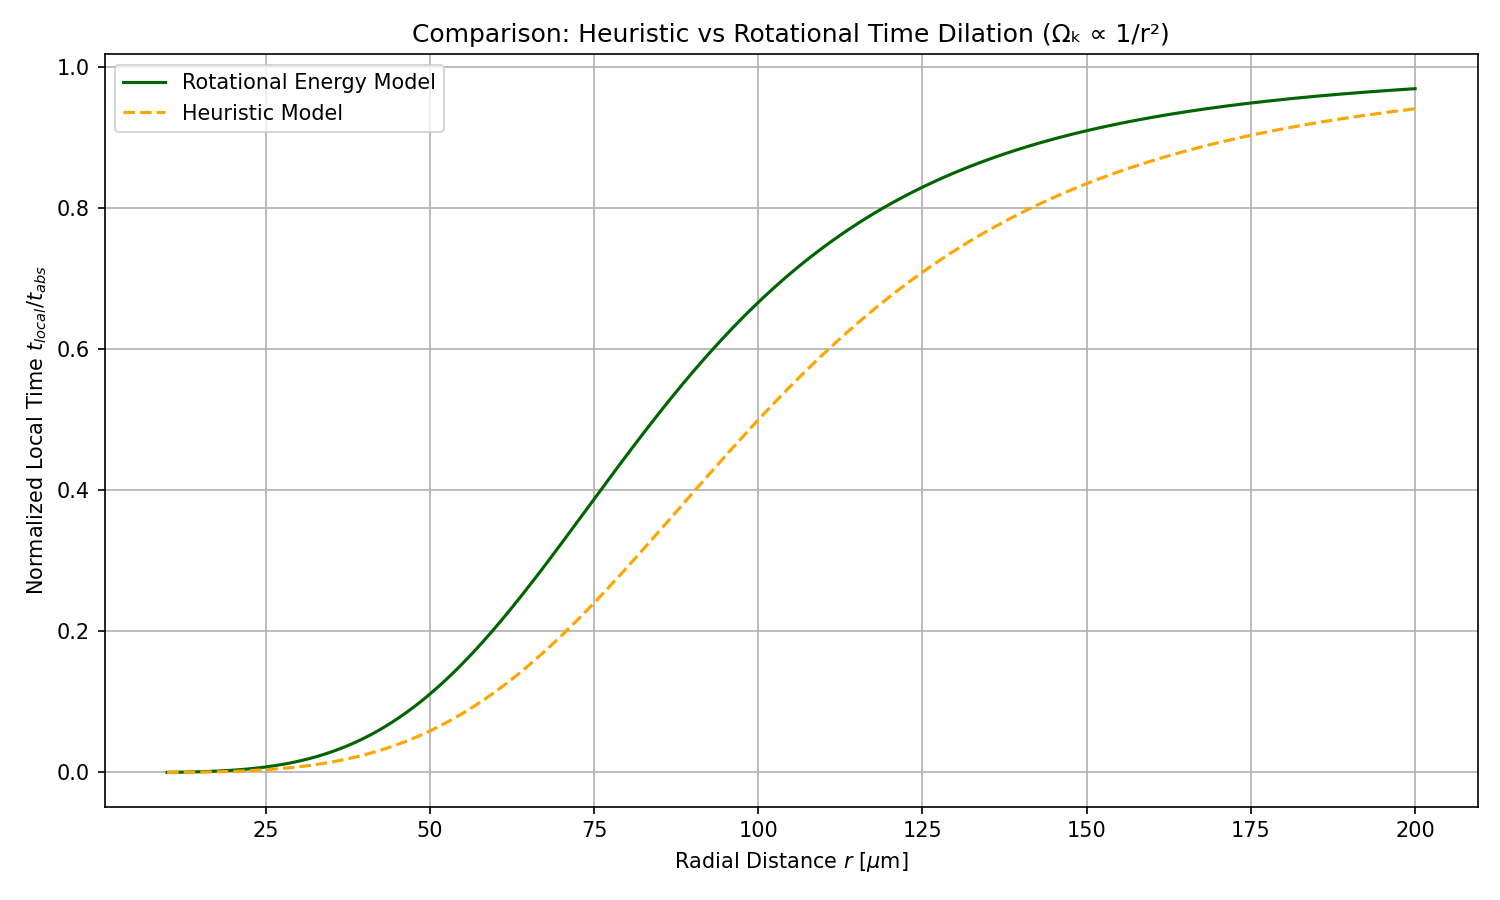
\includegraphics[width=0.7\linewidth]{RotationalVsHeuristicTimeDilation}
    \caption{Verschil tussen VAM en GR-tijddilatatie voor een neutronenster ($2\,M_\odot$, $R=10$ km).}
    \label{fig:vergelijkingVAMGR}
\end{figure}

\subsection{Interpretatie van schaalafhankelijke ætherdichtheid}

VAM gebruikt een schaalafhankelijke ætherdichtheid: lokaal zeer hoog ($\sim10^{18}$ kg/m³) voor kernstabiliteit en macroscopisch laag ($\sim10^{-7}$ kg/m³) om inertievrije propagatie van interacties mogelijk te maken. De hoge dichtheid in wervelkernen versterkt lokaal de wervelsnelheid en daarmee de tijddilatatie significant, terwijl macroscopisch juist minimale weerstand voor propagatie van effecten geboden wordt.

\subsection{Praktische implicaties en experimentele toetsbaarheid}

Een praktische implicatie van wervel-geïnduceerde tijddilatatie is dat klokken dicht bij intense wervelvelden meetbaar trager zouden lopen. Dit kan theoretisch getoetst worden met ultra-precieze atoomklokken in laboratorium wervelexperimenten, of indirect via astrofysische observaties van pulsars en neutronensterren. Het Hafele–Keating experiment biedt een directe analogie voor tijddilatatie door beweging en hoogteverschillen, die in VAM overeenkomt met lokale wervelvariaties~\cite{hafele1972around}.
